% --- Template for thesis / report with tktltiki2 class ---
% 
% last updated 2013/02/15 for tkltiki2 v1.02

\documentclass[finnish]{tktltiki2}

% tktltiki2 automatically loads babel, so you can simply
% give the language parameter (e.g. finnish, swedish, english, british) as
% a parameter for the class: \documentclass[finnish]{tktltiki2}.
% The information on title and abstract is generated automatically depending on
% the language, see below if you need to change any of these manually.
% 
% Class options:
% - grading                 -- Print labels for grading information on the front
%page.
% - disablelastpagecounter  -- Disables the automatic generation of page number
%information
%                              in the abstract. See also
%\numberofpagesinformation{} command below.
%
% The class also respects the following options of article class:
%   10pt, 11pt, 12pt, final, draft, oneside, twoside,
%   openright, openany, onecolumn, twocolumn, leqno, fleqn
%
% The default font size is 11pt. The paper size used is A4, other sizes are not
%supported.
%
% rubber: module pdftex

% --- General packages ---

\usepackage[utf8]{inputenc}
\usepackage[T1]{fontenc}
\usepackage{lmodern}
\usepackage{microtype}
\usepackage{amsfonts,amsmath,amssymb,amsthm,booktabs,color,enumitem,graphicx}
\usepackage[pdftex,hidelinks]{hyperref}

% Automatically set the PDF metadata fields
\makeatletter
\AtBeginDocument{\hypersetup{pdftitle = {\@title}, pdfauthor = {\@author}}}
\makeatother

% --- Language-related settings ---
%
% these should be modified according to your language

% babelbib for non-english bibliography using bibtex
\usepackage[fixlanguage]{babelbib}
\selectbiblanguage{finnish}

% add bibliography to the table of contents
\usepackage[nottoc]{tocbibind}
% tocbibind renames the bibliography, use the following to change it back
\settocbibname{Lähteet}

% --- Theorem environment definitions ---

\newtheorem{lau}{Lause}
\newtheorem{lem}[lau]{Lemma}
\newtheorem{kor}[lau]{Korollaari}

\theoremstyle{definition}
\newtheorem{maar}[lau]{Määritelmä}
\newtheorem{ong}{Ongelma}
\newtheorem{alg}[lau]{Algoritmi}
\newtheorem{esim}[lau]{Esimerkki}

\theoremstyle{remark}
\newtheorem*{huom}{Huomautus}


% --- tktltiki2 options ---
%
% The following commands define the information used to generate title and
% abstract pages. The following entries should be always specified:

\title{OWL - Web Ontology Language}
\author{Hansi Keijonen}
\date{\today}
\level{Seminaariraportti}
\abstract{Tiivistelmä.}

% The following can be used to specify keywords and classification of the paper:

\keywords{avainsana 1, avainsana 2, avainsana 3}
\classification{} % classification according to ACM Computing Classification
%System (http://www.acm.org/about/class/)
                  % This is probably mostly relevant for computer scientists

% If the automatic page number counting is not working as desired in your case,
% uncomment the following to manually set the number of pages displayed in the
%abstract page:
%
% \numberofpagesinformation{16 sivua + 10 sivua liitteissä}
%
% If you are not a computer scientist, you will want to uncomment the following
%by hand and specify
% your department, faculty and subject by hand:
%
% \faculty{Matemaattis-luonnontieteellinen}
% \department{Tietojenkäsittelytieteen laitos}
% \subject{Tietojenkäsittelytiede}
%
% If you are not from the University of Helsinki, then you will most likely want
%to set these also:
%
% \university{Helsingin Yliopisto}
% \universitylong{HELSINGIN YLIOPISTO --- HELSINGFORS UNIVERSITET --- UNIVERSITY
%OF HELSINKI} % displayed on the top of the abstract page
% \city{Helsinki}
%


\begin{document}

% --- Front matter ---

\maketitle        % title page
\makeabstract     % abstract page

\tableofcontents  % table of contents
\newpage          % clear page after the table of contents


% --- Main matter ---

\section{Semanttinen web}
Suurin osa tämän päivän webin sisällöstä on tarkoitettu ihmisten luettavaksi
sekä tulkittavaksi. Kone pystyy tulkitsemaan esim. html-tiedoston ja esittämään
dokumentin siinä määritellyllä tavalla. Ongelma on, että kone ei
\textit{ymmärrä} dokumentin sisällön merkitystä, semantiikkaa \cite{BHL01}.Se,
että kone ei ymmärrä dokumenttien semanttisia merkityksiä rajoittaa esimerkiksi
haut internetissä olevista dokumenteista yksinkertaiseksi hakusanojen
etsimiseksi. Sen sijaan jos hakukoneet ymmärtäisivät asioiden merkityksen ja
niiden välillä vallitsevat yhteydet, olisi hakukoneiden hakutulokset tarkempia
ja sisältäisivät mahdollisesti laajennettuja hakuja alkuperäisen asian ympäriltä
\cite{BHL01}. On siis tarve olla menetelmä  käsitteiden luomiseen, käsitteiden
ominaisuuksien kuvaamiseen sekä käsitteiden välisten suhteiden kuvaamiseen
\cite{BHL01}. Tim Berners-Lee, James Hendler ja Ora Lassila toteavat
artikkelissaan "Semantic web", että "semanttinen web ei ole erillinen web vaan
laajennos tämänhetkiseen webiin, jossa informaatiolle on annettu hyvin muotoiltu
merkitys mahdollistaen koneiden ja ihmisten paremman yhteistyön."  web of
documents -> web of data dataa voi parsia manuaalisesti tai koneellisesti

\section{Teknologiat ja kielet jotka mahdollistavat OWL:n}
W3c tarjoaa semanttisen webin toteuttamiseen standardit teknologioista ja
kielistä. Kuvassa \ref{stack} on semanttisen webin teknologiapino sekä ajatuskonsepteja
semanttisen webin toteuttamiseen. Osa teknologioista on todellisuutta ja
käytössä, osa vasta ideatasolla. Jokainen kerros käyttää alemman kerroksen
palveluita. Seuraavissa kappaleissa käyn läpi kaavion teknologioita ja kieliä
alhaalta ylöspäin kohti OWL:ää. Jokaisesta seuraavissa kappaleissa esitetystä
teknologiasta käsitellään tarkemmin ne konstruktiot, jotka ovat olennaisia ja käytössä 
myös OWL:ssä.

\begin{figure}[h]
 \centering
 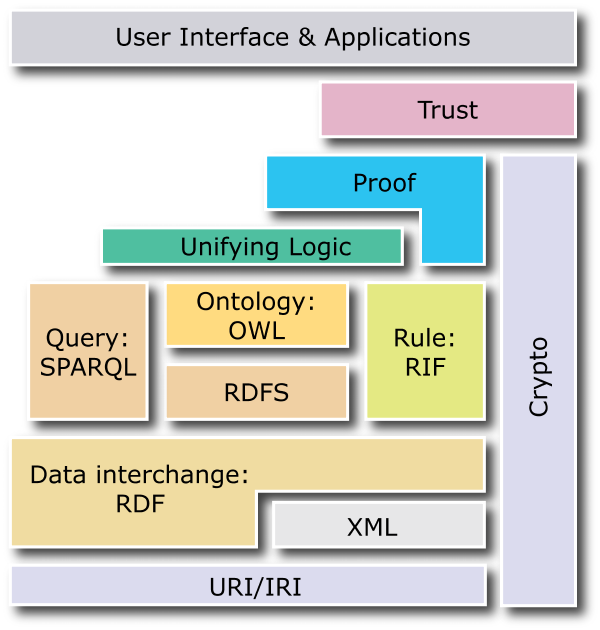
\includegraphics[scale=0.50]{stack.png}
 \caption{Semanttisen webin toteutukseen tarvittavat teknologia, kielet ja konseptit. }
 \label{stack}
\end{figure}
 
\subsection{URI ja XML}

Semanttisessa webissä luokkia, ilmentymiä, ominaisuuksia ja ominaisuuksien
arvoja kutsutaan resursseiksi. Jotta sekaannusta jo määritettyjen resurssien
sekä uusien määritysten kanssa ei syntyisi, identifioidaan kaikki resurssit (pl.
ominaisuuksien literaaliarvot) yksilöllisesti URI(Unified Resource Locator):lla.
URI:n avulla voidaan viitata mihin tahansa määritettyyn resurssiin. Useinmiten
URIna toimii perinteinen URL(Unified Resourse Locator)-osoite \cite{BHL01}. IRI
(Internationalized Resource Identifier) on ainoastaan merkistölaajennos URI:in.
 
Semanttisen webin datan kuvaukset toteutetaan useimmiten XML-tiedostoina.
XML-kieltä voidaan käyttää monimutkaisen rakenteisen tiedon esittämiseen ja
tarjoaa näin standardoidun mallin tiedon vaihtamiseen prosessoijien välillä.
Tärkeä XML:n ominaisuus on nimiavaruudet, jotka mahdollistavat resurssien
identifioinnin URI:en avulla. Tästä kuitenkin enemmän seuraavissa kappaleissa. 

\subsection{Tiedon esittäminen RDF-triploilla}

Resource Description Framework RDF on kieli webissä olevien resurssien
kuvaamiseen. 
RDF perustuu asioiden identifiointiin URI:lla ja näiden asioiden kuvaamiseen 
ominaisuuksilla ja ominaisuuksien arvoilla. Tämä mahdollistaa yksinkertaisten
lausumien 
esittämisen verkkoina, joissa resurssit ja ominaisuudet ovat soluja ja
ominaisuudet verkon 
kaaria \cite{RDFP}. Kuvassa \ref{jack} on havainnollistettu asiaa. 

\begin{figure}[h]
 \centering
 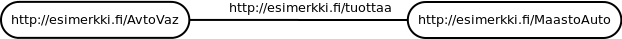
\includegraphics[scale=0.50]{JackTorrance.png}
 \caption{RDF-tripla joka kuvaa yksinkertaisen lausuman. Jokainen triplan solmu
ja kaari on identifioitu URI:lla. }
 \label{jack}
\end{figure}

Kuvassa \ref{jack} on havainnollistettu yksinkertainen \textit{RDF-tripla}.
Triplan 
subjekti, predikaatti ja objekti kertovat, että "Jack Torrance on ammatiltaan
kirjailija".
Jokainen solu ja kaari on esimerkissä identifioitu URI:lla. Objekti voi olla
myös literaali, jolloin 
sitä ei identifioida erikseen, mutta formaatti määritellään ****NIIN VITTU
MILLÄ?*****

Yleisin tapa esittää tripla on XML-notaatio. Myös muut tavat ovat mahdollisia,
kuten 
esimerkiksi \textit{JSON} ja \textit{turtle}. Alla on esitetty kuvassa
\ref{jack} triplan XML-notaatio:
\begin{verbatim}
<rdf:Description rdf:about="http://example.org/JackTorrance">
    <rel:HasProfession rdf:resource="http://example.org/Author"/>
</rdf:Description>
\end{verbatim}

Esimerkistä näkee selvästi, kuinka subjekti, predikaatti ja objekti ovat
identifioitu
URI:lla. Jack Torrance on toiselta ammatiltaan talonmies ja myös Laila Hietamies
on 
ammatiltaan kirjailija. Kun myös nämä triplat kuvataan samaan kaavioon, alkaa
pieni 
mutta informatiivinen verkkkuva ja selitys triploista ja URI:sta? Kyllä, tähän se sopisi kokoavana
elementtinä.
o syntyä, kuva \ref{jack2}. Tästä verkosta voisimme
tehdä hakuja, kuten 
"ketkä ovat kirjailijoita?".

\begin{figure}[h]
 \centering
 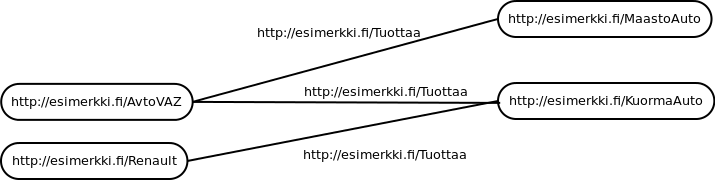
\includegraphics[scale=0.50]{torrance2.png}
 \caption{RDF-triplat muodostavat verkon.}
 \label{jack2}
\end{figure}

RDF:n peruskonstruktioita ovat: description, resource, about ***selitä nää*****

RDF tarjoaa siis vain melko alkeellisen tavan esittää lausumia, jotka
muodostavat haut mahdollistavan verkon. RDF toteuttaa myös joukon muita ominaisuuksia, kuten
\textit{säiliöitä} (container) tiedon säilömiseen sekä
\textit{kokoomatietorakenteita}
(collections) asioiden listaamiseen \cite{RDFP}. Näitä käsitellään myöhemmin
niiltä osin 
kuin ne ovat relevantteja OWL-ontologioiden muodostamisessa.  
 
\subsection{Alkeelliset ontologiat RDF Schemalla}
Semantiikkaa voidaan webissä ilmaista ontologioilla. Tietojenkäsittelytieteessä
ontologialla tarkoitetaan dokumenttia, jossa kerrrotaan asioiden välisistä
yhteyksistä \cite{BHL01}. ***vajaa läppä!! kuuluuko edes tähän???!!*******

RDF:llä ilmaistut ominaisuudet voidaan ajatella resurssien attribuuteiksi
samassa mielessä kuin perinteiset attribuutti-arvo -parit \cite{RDFS}. Vaikka 
RDF:llä voidaan kuvata resursseja, se ei tarjoa keinoja kuvata ominaisuuksia tai
ominaisuuksien välisiä suhteita. Tämä on mahdollista RDF:n \textit{sanastonkuvauslaajennoksella}
RDF Schemalla. RDF Schemalla on mahdollista määritellä luokkia ja ominaisuuksia
joita voidaan käyttää luokkien, ominaisuuksien ja resurssien kuvaamiseen \cite{RDFS}. 
RDF Schema on RDF:n semanttinen laajennos. 

Seuraavassa esitellään RDF Scheman niitä peruskonstruktioita, 
joita myös OWL käyttää määrittelyssään lähes sellaisenaan. \emph{RDFS Schema määrittelee myös suurehkon joukon muita konstruktioita, mutta niiden esittely OWL:n selostamisen kannalta on tässä tarpeetonta.} 

\subsubsection{Luokat ja ilmentymät}
Resurssit voidaan jaotella luokkiin. Luokkien jäseniä nimitetään luokan ilmentymiksi \cite{RDFS}. Luokat ovat itsessään resursseja. Useimmiten luokat identifioidaan RDF:n URI:lla ja niitä voidaan kuvata RDF:n ominaisuuksilla (property). Luokka ilmaistaan rdfs:Class tagilla, rdf:type ominaisuudella voidaan ilmaista, että resurssi kuuluu luokkaan \cite{RDFS}. Esimerkiksi kustannusosakeyhtiö "WSOY" on itse luokka ja  luokan "Kustantamo" ilmentymä:
\begin{verbatim}
Esim:WSOY rdf:type rdfs:Class
Esim:WSOY rdf:type esim:Kustantamo
\end{verbatim}  

\subsubsection{Luokan aliluokka}
rdfs:subClassOf ominaisuudella voidaan ilmaista, että jonkin luokan ilmentymät ovat myös jonkin toisen luokan ilmentymiä \cite{RDFS}. Esimerkiksi 
luokka "Kustantamo" on luokan "Liikeyritys" aliluokka:
\begin{verbatim}
esim:Kustantamo rdfs:subClassOf esim:Liikeyritys 
\end{verbatim}

\subsubsection{Ominaisuudet ja periytetyt ominaisuudet}
Resursien välisiä suhteita kuvataan ominaisuuksilla. Esimerkiksi "Matilla on veli Teppo". Voidaan ajatella, että resurssien "Matti" ja "Teppo" välinen suhde on ominaisuus "Veljeys". Ominaisuus "Veljeys" voi olla ominaisuuden "Perhesuhde"  aliluokka tai paremminkin aliominaisuus. Tällaisia konstruktioita kuvataan RDF Schemassa termillä subPropertyOf: 
\begin{verbatim}
esim:Veljeys rdfs:subPropertyOf esim:Perhesuhde
\end{verbatim}
 subPropertyOf ilmaisee määritelmällisesti, että resurssit joiden välistä suhdetta kuvataan jollain suhteella, voidaan kuvata myös tämän suhteen ylisuhteella, josta ko. suhde on periytynyt \cite{RDFS}. 
\subsubsection{Rajoitukset ominaisuuksien sovellusalueissa ja arvoissa}
RDF Schemassa on mahdollista antaa ominaisuuksille rajoituksia sen suhteen, että minkä luokkien välistä suhdetta ominaisuus kuvaa. Ensinnäkin
voidaan rajoittaa suhteen sovellusaluetta (domain). Suhteen  "Työskentelee" sovellusalue voidaan rajata koskemaan ainoastaan luokkaa "Työntekijä". Samaten suhteen saamat arvot (range) voidaan rajata olemaan ainoastaan luokan "Yritys" tai sen aliluokkien ilmentymiä. 
\begin{verbatim}
esim:Työskentelee rdfs:domain esim:Työntekijä
esim:Työskentelee rdfs:range esim:Yritys
\end{verbatim}

\subsubsection{RDF Schema esimerkki}
Myös RDF Scheman varsinainen notaatio on toteutettu XML:llä. Alla on lyhyt esimerkki RDF Schemalla toteutetusta ontologiasta.: 
\begin{verbatim}
<?xml version="1.0"?>
<rdf:RDF
xmlns:rdf="http://www.w3.org/1999/02/22-rdf-syntax-ns#"
xmlns:rdfs="http://www.w3.org/2000/01/rdf-schema#"

<rdfs:Class rdf:ID="liikeyritys" />

<rdfs:Class rdf:ID="kustantamo">
  <rdfs:subClassOf rdf:resource="#liikeyritys"/>
</rdfs:Class>

</rdf:RDF>
\end{verbatim}

Esimerkissä on yksinkertainen ontologia, joka kertoo, että "kustantamo" ja "liikeyritys" ovat luokkia ja että "kustantamo" on myös luokan "liikeyritys" aliluokka. RDF Schema  -ontologiat ovat RDF-tiedostoja samoin kuin OWL-ontologiatkin. Tiedoston alussa olevat nimiavaruusmäärittelyt varmistavat, että rdf- ja rdfs-alkuisilla tageilla ympäröidyt elementit todellakin ovat rdf- ja rdfs- elementtejä. Nimiavaruudet käsitellään takemmin OWL:n esittelyn yhteydessä. 

\section{Kehittyneitä ontologioita OWL:llä}



Tälä hetkellä kehittynein tapa ilmaista ontologioita on OWL-ontologiat. Lyhenne OWL tulee 
sanoista Web Ontology Language. Vaikka määritelmässä on sana language, kieli, on 
OWL-ontologiat ymmärettävä ennemminkin sanastoina, joita on kuvattu RDF-kielellä.
 Eräs tapa hahmottaa RDF-triplojen ja
OWL-ontologioiden välinen ero on verrata niitä perinteiseen
relaatiotietokantaan. RDF-triplat on tapa tallettaa tietoa olioiden ominaisuuksista samalla tavalla kuin
relaatiotietokannan taulun riveillä tallennetaan rakenteista tietoa tietokantaolioista. Jokaista riviä relaatiotietokannassa
yksilöi yksilöivä avain kun taas RDF-triploissa avaimen virkaa hoitaa URI. Relaatiotietokannoissa tietokantaolion attribuuttien suhteita ilmaistaan taulurakenteilla ja tietokantaolioiden suhteita toisiin tietokantaolioihin ilmaistaan viitteillä taulujen välillä. Vastaavasti voidaan ajatella, että OWL-ontologiat kuvaavat ja jäsentävät  samalla tavalla RDF-triploilla ilmaistua tietoa: ontologialla voidaan määritellä monipuolisesti luokkien, ilmentymien ja suhteiden ominaisuuksia.  RDF on kuin kieli jolla ilmaistaan lausumia asioista kun taas OWL on sanasto, jonka avulla lausumien merkitykset ymmärretään. 

OWL tarjoaa ontologioiden määrittelyyn \cite{AH09} 
\begin{itemize}
\item \textit{hyvin määritellyn syntaksin} , jotta ontologiat olisivat koneluettavissa
\item \textit{hyvin määritellyn semantiikan}, jolla voi ilmaista merkityksiä tarkasti ja konsistentisti
\item \textit{tuen koneelliselle päättelylle}, jotta esim.  ontologioiden eheys voidaan tarkastaa automaattisesti
\item \textit{riittävästi ilmaisuvoimaa} ilmaisemaan kaikki tarvittavat merkitykset
\item \textit{miellyttävän ilmaisutavan}, jotta työskentely olisi sujuvaa
\end{itemize}


Ideaalisesti OWL on RDF:n ja RDF Scheman laajennos \cite{AH09}. OWL käyttää
RDF:n luokkia ja suhteita lisäten niihin omia laajennoksiaan. RDF Schemassa on joitain 
hyvin vahvoja konstruktioita, kuten rfd:Class
(kaikkien luokkien yliluokka) sekä rdf:Property (kaikkien suhteiden yliluokka).
Näiden primitiivien ilmaisuvoima yhdistettynä OWL:n tarjoamaan laajennoksiin
on ristiriidassa sen tavoitteen kanssa, että ontologiat olisivat koneellisesti
pääteltävissä. Tämä tasapainotila mielessäpitäen on määritelty kolme OWL:n
alikieltä sen perusteella, painotetaanko ilmaisuvoimaa vai koneellista päättelyä
\cite{AH09}.  

\subsection{OWL:n kolme alikieltä}

W3C:n Web Ontology Working Group on määritellyt OWL:lle kolme alikieltä, joiden
on takoitus toteuttaa eri aspektit (ilmaisuvoima, koneellinen päättely), joita
ontologioiden kuvaamiskieleltä vaaditaan \cite{MH04}. Alikielet ovat ilmaisuvoiman mukaisesti
kasvavassa järjestyksessä:

\begin{itemize}
 \item \textit{OWL Lite} tarjoaa ainoastaan yksinkertaisen luokitteluhierarkian ja yksinkertaiset rajoitteet\cite{MH04}. Kardinaalisuusrajoitteet ovat ainoastaan muotoa 0 ta 1. Työkalutuen tarjoaminen on OWL Litelle helpompaa kuin ilmaisuvoimaisemmille versioille \cite{MH04}.  
 \item \textit{OWL DL} on tarkoitettu niille käyttäjille, jotka haluavat mahdollisimman hyvän ilmaisukyvyn siten, että ontologia on koneellisesti pääteltävissä (kaikki päätelmät tehtävissä järjellisessä ajassa) \cite{MH04}. OWL DL tarjoaa kaikki kielen konstruktiot, mutta niitä voi käyttää tietyin rajoituksin, esimerkiksi luokka voi olla monen luokan aliluokka mutta ei voi olla samalla luokan ilmentymä. DL tulee sanoista Description Logics, deskriptiivinen logiikka, joka on tieteenala, joka tutkii logiikkaa ja on OWL:n perusta \cite{MH04}.  
 \item \textit{OWL Full} on tarkoitettu niille käyttäjille, jotka haluavat maksimaalisen ilmaisukyvyn välittämättä siitä, onko ontologiat enää koneellisesti pääteltävissä \cite{MH04}. Toisin kuin OWL DL:ssä, luokka voi olla kokoelma yksilöitä (instansseja) samalla kuin luokka itsessään on jonkin luokan yksilö. OWL Full mahdollistaa jo olemassa olevien ontologioiden laajentamisen. On epätodennäköistä, että mikään ohjelmisto pystyy täydellisesti päättelemään OWL Full ontologioita \cite{MH04}. 
\end{itemize}

%Edellisissä kappaleissa on valotettu RDF:n ja RDF Scheman keinoja ilmaista merkityksiä.
%RDF/RDF Schemassa on toteutettu luokkien ja ominaisuuksien hierarkinen järjestelmä, ominaisuuksien sovellusalue ja
%arvorajoitukset sekä luokkien ilmentymien väliset suhteet \cite{AH09}. Mutta
%useita tarpeellisia ominaisuuksia puuttuu, jotka on toteutettu OWL:ssä,
%esimerkiksi \cite{AH09}:
%\begin{itemize}
% \item \textit{Rajoitukset suhteen kohteessa}: (WTF?) RDFS:ssä voidaan
%määritellä rajoituksia, mitä arvoja tai muita luokkia suhteen objektiksi voidaan
%asettaa. Kuitenkaan ei ole mahdollista määrätä rajoitteita sen suhteen, onko
%jotkut rajoitteet voimassa vain rajatulle joukolle luokkia. 
% \item \textit{Luokkien poissulkevuus}: joissain tapauksissa on hyvä pystyä
%sanomaan, että joku luokka on poissulkeva toisen luokan suhteen. Voidaan sanoa
%esimerkiksi että luokka 'mies' on poissulkeva suhteessa luokkaan 'nainen'
% \item \textit{Luokkien joukko-operaatiot}: toisinaan on tarve muodostaa uusia
%luokkia olemassaolevien joukkojen perusteella. Esimerkiksi luokka 'henkilö'
%voitaisiin määritellä luokkien 'mies' ja 'nainen' yhdisteeksi kuitenkin niin,
%että henkilö voi olla vain joko mies tai nainen (poissulkevuus).
% \item \textit{Suhteiden kardinaliteetit}: joihinkin suhteisiin on hyvä
%määrittää rajoituksia sen suhteen kuinka monta arvoa arvoksi voi antaa.
%Esimerkiksi ihmisellä voi olla ainoastaan kaksi vanhempaa.
% \item \textit{Suhteiden erikoisominaisuudet}: suhteet voidaan määritellä
%\textit{transitiivisiksi, uniikeiksi} jonkun toisen suhteen
%\textit{inversioksi}. 
%\end{itemize}
%Tarvitaan siis kieli, joka on rikkaampi kuin RDF Schema \cite{AH09}. OWL:n
%suunnittelussa on jouduttu tasapainoilemaan kielen ilmaisuvoiman ja sen
%soveltuvuudesta koneelliseen päättelyyn. Mitä rikkaampi ja ilmaisuvoimaisempi
%kieli on, sitä hankalampi ja tehottomampi sen pohjalta on päätellä asioita.
%Pahimmassa tapauksessa päättely muodostuu mahdottomaksi tehtäväksi \cite{AH09}. 

\subsection{OWL-ontologian rakenne}

\subsubsection{Nimiavaruudet}
XML-dokumentissa tulee määritellä nimiavaruudet (namespace). Nimiavaruuksien
avulla voidaan ratkaista mm. samannimisten elementtien aiheuttamia
tulkintaongelmia sekä kertoa lukijalle (koneelle tai ihmiselle) konteksti, jonka
mukaan elementtien tageja tulee tulkita. OWL-ontologiassa nimiavaruudet
määritellään rdf:RDF -kahvojen sisään. \textit{Kaikki OWL-ontologiat ovat RDF-dokumentteja} \cite{SWM04}. Alla olevassa esimerkissä on eräs mahdollinen nimiavaruusmäärittely . 
\begin{verbatim}
<rdf:RDF 
    xmlns:esim ="http://www.esimerkki.com/esim#" 
    xmlns:owl ="http://www.w3.org/2002/07/owl#"
    xmlns:rdf ="http://www.w3.org/1999/02/22-rdf-syntax-ns#"
    xmlns:rdfs="http://www.w3.org/2000/01/rdf-schema#"
    xmlns:xsd ="http://www.w3.org/2001/XMLSchema#">
\end{verbatim}
Esimerkin nimiavaruusmäärittelyissä on määritelty nimiavaruus niille tageille, jotka käyttävät etuliitettä esim:. 
Nimiavaruudet on määritelty myös owl:-, rdf:- ja rdfs:-etuliiteille kertomaan, että näillä
etuliitteillä varustetut tagit edustavat OWL:n, RDF:n ja RDF Scemann termistöä.
OWL-ontologia on riippuvainen myös XMLSchema-datatyypeistä (xsd:), joten myös niiden
nimiavaruus tulee määrittää. 

\subsection{Otsikkotiedot}
Owl-ontologian otsikkotiedoissa voidaan kertoa yleisiä asioita kuten versiotietoa, kommentteja, ontologian nimi sekä
tärkeänä ominaisuutena importata muita ontologioita. Otsikkotiedot määritellään owl:Ontology-elementiksi: 
\begin{verbatim}
<owl:Ontology>
   <rdfs:label>Esimerkkiontologia</rdfs:label>
   <rdfs:comment>Esimerkin voimaa</rdfs:comment>
   <owl:priorVersion>
       rdf:resource="http://www.esimerkki.com/vanhempi#"
   </owl:priorVersion>
   <owl:imports>rdf:resource="http://purl.org/dc/elements/1.1"</owl:imports>
</owl:Ontology>
\end{verbatim}
Esimerkkiotsikossa perustietojen lisäksi importataan Dublin Core - sanasto  \footnote{Dublin Core on nnnnn}  ontologiamme käyttöön.

\subsection{Yksinkertaiset luokat ja aliluokat}
OWL:ssä kaikki yksilöt ovat luokan owl:Thing jäseniä ja kaikki käyttäjän määrittämät luokat owl:Thingin aliluokkia \cite{SWM04}. Myös owl:Nothing on määritelty(MIX VITUSCH?). Luokkamäärittelyt tapahtuvat hyvin samaan tapaan kuin RDF Schemassa, ainoastaan tagin nimi on owl:Class. Aliluokkanotaatio vastaa suoraan RDF Scheman konstruktiota:
\begin{verbatim}
<owl:Class  rdf:ID="Auto">
<owl:Class  rdf:ID="Ajoneuvo">

<owl:Class rdf:ID="Auto">
    <rdfs:subClassOf rdf:resource="Ajoneuvo"/>
</owl:Class>
\end{verbatim}
Esimerkissä on määritetty kaksi luokkaa "Auto" ja "Ajoneuvo" sekä määritelty edellinen jälkimmäisen aliluokaksi. 

OWL:ssä on myös mahdollista määritellä luokka siten, että luokan jäsenet voivat kuulua ko. luokkaan mutta eivät missään tapauksessa
implisiittisesti määritettyyn toiseen luokkaan:
\begin{verbatim}
<owl:Class ref:about="Ajoneuco">
    <owl:disjointWith rdf:resource="Elain"
</owl>
\end{verbatim}
Luokan "Ajoneuvo" ja sen mahdollisten aliluokkien jäsenet eivät voi siis kuulua samaan aikaan luokkaan "Kissa" tai sen mahdollisiin aliluokkiin. Voidaan siis päätellä, että ilmentymä "Lada" ei voi olla luokan "Kissa" jäsen jos "Kissa" on määritetty luokan "Eläin" aliluokaksi. 

\subsection{Luokan yksilöt}
Luokan jäseniä kutsutaan yksilöiksi, eli luokan ilmentymiksi \cite{SWM04}. Jonkun ilmentymän kuuluminen luokkaan ilmaistaan samalla tavalla kuin RDF Schemassa rdf:type konstruktiolla. Ensiksi määritellään kuitenkin instanssi owl:Thing-tagilla:
\begin{verbatim}
<owl:Thing rdf:ID="Lada"/>

<owl:Thing ref:about="Lada">
    <rdf:type= rdf:resource="Autonvalmistaja"/>
</owl:Thing>
\end{verbatim}
Esimerkissä määritettiin "Autonvalmistaja"-luokan ilmentymä "Lada". Esimerkissä viitataan oletetusti jo aiemmin määritettyyn "Autonvalmistaja"-luokkaan \cite{SWM04}. 

\subsection{Luokkaominaisuus ja datatyyppiominaisuus}
Ominaisuudet jaetaan OWL:ssä luokkaominaisuuksiksi (Object Property) ja datatyyppiominaisuuksiksi (Data Type Property) sen perusteella liittääkö ominaisuus yhteen kaksi luokan ilmentymää vai luokan ilmentymän ja RDF-literaalin tai XML Schema -datatyypin  \cite{SWM04}. 
\subsubsection{Luokkaominaisuus}
OWL:ssä luokkaominaisuudet määritellään kuten mitkä tahansa luokat, mutta käyttäen ObjectProperty -konstruktiota. Määrittelyssä kerrotaan myös minkä luokan ilmentymiin ominaisuus on sovellettavissa sekä mitä arvoja (luokkia) ominaisuus voi saada. Nämä rajoitteet ilmaistaan RDF Schemasta tutuilla rdfs:domain- ja rdfs:range-elementeillä:
\begin{verbatim}
<owl:ObjectProperty rdf:about="Merkki"/>

<owl:ObjectProperty rdf:ID="Merkki">
    <rdfs:domain rdf:resource="Auto"/>
    <rdfs:range rdf:resource="Autonvalmistaja"/>
</owl:ObjectProperty>
\end{verbatim}
Esimerkissä on määritelty ominaisuus "Merkki", jolla voi kuvata ainoastaan luokan "Auto" ilmentymiä ja joka voi ainoastaan saada arvokseen ainoastaan luokan "Autonvalmistaja" ilmentymiä. 

\subsubsection{Datatyyppiominaisuus}
Datatyyppiominaisuus liittää yhteen luokan ilmentymän ja datan arvon: RDF-literaalin tai XML Schema -datatyypin. Myös datatyyppiominaisuuksien määrittelyssä kerrotaan minkä luokan ilmentymiin ominaisuus on sovellettavissa sekä minkä tyyppisiä arvoja ominaisuus voi saada \cite{SWM04}. Rajoitteet tehdään samalla tavalla kuin luokkaominaisuuden määrittelyssä:
\begin{verbatim}
<owl:DataTypeProperty rdf:about="Valmistusvuosi"/>

<owl:DataTypeProperty rdf:ID="Valmistusvuosi">
    <rdfs:domain rdf:resource="Auto"/>
    <rdfs:range  rdf:resource="&xsd;gYear"/>   
<owl:dataTypeProperty>
\end{verbatim}
Esimerkissä määritetään ominaisuus "Valmistusvuosi", jolla voidaan kuvata luokan "Auto" ilmentymiä ja joka voi saada arvokseen XML Schema -standardissa määritetyn gYear-tyypin arvon. XML-Schema -standardi määrittelee kymmeniä eri datatyyppejä XML-dokumenteissa käytettäväksi. Kun käytetään määritettyjä datatyyppejä, XML-parseri pystyy tarkistamaan, onko annetut arvot sallittuja ja esitystapa oikea.  

\subsubsection{Aliominaisuudet}
Myös ominaisuuksille voidaan määritellä aliominaisuuksia samaan tapaan kuin luokille voidaan määrittää aliluokkia. Aliominaisuus toteutetaan subPropertyOf-konstruktiolla, joka on toteutettu jo RDF Schemassa \cite{SWM04}. Alla olevassa esimerkissä lisätään ominaisuuteen "Valmistusvuosi" määritys, että se on ominaisuuden "AutonKuvailija" aliominaisuus:
\begin{verbatim}
<owl:Class rdf:ID="AutonKuvailija">

<owl:DataTypeProperty rdf:ID="Valmistusvuosi">
    <rdfs:subPropertyOf rdf:resource="AutonKuvailija">
    . . .
<owl:dataTypeProperty>
\end{verbatim}

\subsubsection{Kardinaalisuusrajoitteet}
OWL antaa mahdollisuuden määrätä kardinaalisuusrajoitteita ominaisuuksien arvoille kun ominaisuutta sovelletaan tietyssä kontekstissa \cite{SWM04}. Voidaan esimerkiksi määrätä, että luokka "Ajoneuvo" on joukko asioita, joilla on aina vähintään kaksi "Renkaat"-ominaisuutta. ***KIRJOITA SELKEÄMMIN TOI*** Tämä määritetään siten, että luokalle "Ajoneuvo" määritetään anonyymi aliluokka, jolle kardinaalisuusrajoite annetaan. Alla oleva esimerkki selventää asiaa:
\begin{verbatim}
<owl:Class  rdf:ID="Ajoneuvo">
    <rdfs:subClassOf>
       <owl:Restriction>
           <owl:onProperty rdf:resource="Renkaat"
           <owl:minCardinality rdf:datatype="&xsd;nonNegativeInteger">2
           </owl:minCardinality>
       </owl:Restriction>
    </owl:subClassOf>
<owl:Class/>
\end{verbatim}
Anonyymi aliluokka määrätään normaalilla subClassOf-konstruktiolla. Aliluokalle määritetään rajoite owl:Restriction-tagilla ja kardinaalisuusrajoite tässä tapauksessa  minCardinality-elementillä. Kardinaalisuus määritetään koskemaan ominaisuutta "Renkaat" onProperty-elementillä. Kardinaalisuusrajoitteita voi määrätä myös maxCardinality-elementillä, joka määrää suhteen yläkardinaliteetin, sekä Cardinality-elementillä, joka määrää tarkan arvon mikä on luokan esiintymän ja ominaisuuden suhde. Voitaisiin esimerkiksi määrittää luokka "Moottoripyörä" siten, että seillä voisi olla tasan kaksi "Renkaat" ominaisuutta.   

\subsubsection{Ominaisuuden transitiivisuus, symmetrisyys, funktionaalisuus ja inversio}
Ominaisuuden voi tarvittaessa määrittää transitiiviseksi, symmetriseksi tai funktionaaliseksi \cite{SWM04}. Transitiivinen ominaisuus voidaan määrittää seuraavasti ominaisuudelle P ja ilmentymille x,y ja z \cite{SWM04}:

P(x,y) ja P(y,z) -> P(x,z)

Esimerkiksi omnaisuus rdfs:subClassOf on transitiivinen. Itse määritetyn ominaisuuden voi määrittää transitiiviseksi määrittämällä ominaisuus luokan "TransitiveProperty" jäseneksi:
\begin{verbatim}
. . .
<rdf:type rdf:resource="&owl;TransitiveProperty"
. . .
\end{verbatim}
ESIMERKKI?

Symmetrinen ominaisuus voidaan määrittää ominaisuudelle P ja ilmentymille x,y ja z  \cite{SWM04}:

P(x,y) joss P(y,x)

Vastaavasti oman ominaisuuden voi määrittää symmetriseksi määrittämällä se luokan "SymmetricProperty" jäseneksi:
\begin{verbatim}
. . .
<rdf:type rdf:resource="&owl;SymetricProperty"
. . .
\end{verbatim}
Esimerkiksi ominaisuus "Sisar" voitaisin määritellä symmetriseksi. Jos x on y:n sisar niin implisiittisesti voidaan päätellä, että y on x:n sisar.

Funktionaalinen ominaisuus voiadaan määrittää ominaisuudelle P, ilmentymille x,y ja z  \cite{SWM04}:

P(x,y) ja P(x,z) -> y = z

Edellisten esimerkkien tapaan ominaisuuden voi määrittää funktionaaliseksi:
\begin{verbatim}
. . .
<rdf:type rdf:resource="&owl;FunctionalProperty"
. . .
\end{verbatim}
Funktionaalinen ominaisuus voisi olla esimerkiksi opiskelijanumero. Jokainen opiskelijaluokan ilmentymä, joka olisi myös saman oppilaitoksen jäsen, voitaisiin identifioida opiskelijanumero-ominaisuuden perusteella, koska on olemassa ainoastaan yksi ominaisuuden ilmentymä, jolla on tietty opiskelijanumero.

INVERSIO JA FUNKTIONAALINEN INVERSIO???

   
 










 






\section{OWL2}



% --- Back matter ---
%
% bibtex is used to generate the bibliography. The babplain style
% will generate numeric references (e.g. [1]) appropriate for theoretical
% computer science. If you need alphanumeric references (e.g [Tur90]), use
%
% \bibliographystyle{babalpha-lf}
%
% instead.

\bibliographystyle{babplain-lf}
\bibliography{lahteet}


\end{document}
